\documentclass{amsart} 
\usepackage{graphicx}
\graphicspath{{./}}
\usepackage[fontsize=14pt]{scrextend}
\usepackage{hyperref}
\usepackage{csvsimple}
\usepackage{epigraph}
\title{Universal Human Nature Attitude Towards Corporations}
\author{Zulfikar Moinuddin Ahmed}
\date{\today}
\begin{document}
\maketitle

\section{Opinion About Attitudes Toward Corporations}

Pew 2014 survey of 44 countries.  The analysis here uses $N=35,430$ so the statistics are robust.

% latex table generated in R 4.0.3 by xtable 1.8-4 package
% Wed Apr 14 13:09:10 2021
\begin{table}[ht]
\centering
\begin{tabular}{rrrr}
  \hline
 & x & sx & tf \\ 
  \hline
1 & 0.1712 & 0.0087 &  1 \\ 
  2 & 0.4934 & 0.0115 &  2 \\ 
  3 & 0.2246 & 0.0096 &  3 \\ 
  4 & 0.1107 & 0.0073 &  4 \\ 
   \hline
\end{tabular}
\end{table}

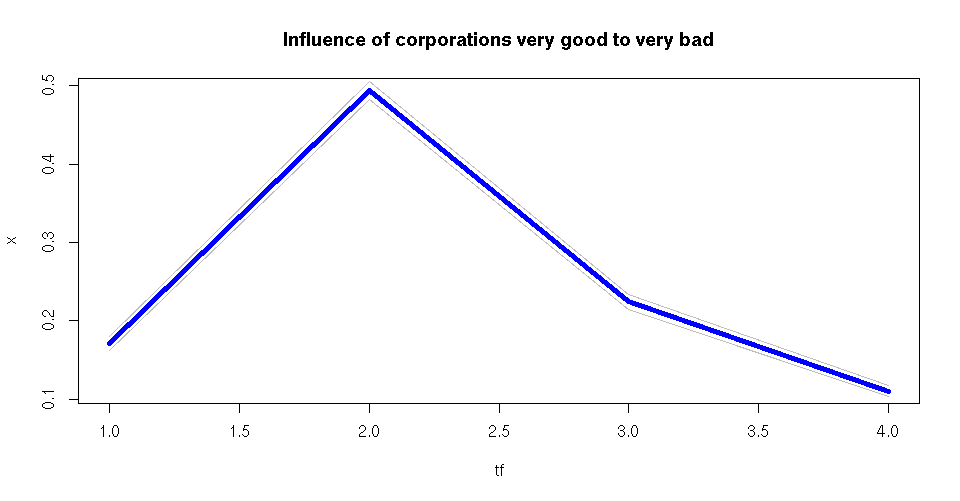
\includegraphics[scale=0.5]{corpop.png}

\section{Interpretation}

A randomly chosen set of people from around the world will have this distribution for their views about corporation effects.  It is not interesting that this is the distribution of opinion at a particular moment but that the standard deviations are so tight that this is the invariant distributions about Human Nature attitude toward corporations.  With this stronger interpretation, we can infer that for deeper reasons than we understand, around 33\% of human race will not like the influence of corporations, and we expect the distribution to be steady.  

These are distributions that we need to simply accept.  A third of humanity will not like influence of corporations, ever. And we have to produce societies which can accept this.  In particular, I do not believe any amount of corporate propaganda will move this 33\% and we have to produce civilisations which accomodate both.

\section{My Commentary}

Around the world, in every nation and religion, we expect that a third of the people will never like corporations.  Now you might, because two-thirds will like corporations, hope that the one-third will accept corporations if only you pressed them or cajoled them or ignored them.  But these are not wise decisions.  The wise decisions will accept that some people, a third, will simply dislike corporations, and arrange society so that they can be accepted as part of society, have meaningful productive lives without having to have corporations shoved down their throats because corporations are liked by majority, and accept that they have a right to have productive fulfilling lives.  In a sense democratic politics makes a good assumption that people ought to voice their opinions and majority will make the right decision.  I am going to be anti-democratic here and say well we know that a third, a nominal minority, will always be shafted, so it is cruel social and political thought that will just be capitalist ideologically.  You must accept that meaningful lives are naturally demanded with productive work and earnings too without corporations for this minority because otherwise you are asking for conflict and my result shows the stability of this phenomena in the Human Race.  
\end{document}